  \documentclass[twoside=true, %  doppelseitiger Druck
    DIV=15
    ,% 11 DIV Faktor für Satzspiegelberechnung - muss bei anderen Schriftgrößen als 11pt angepasst werden , sie Doku zu KOMA Script
    BCOR=15mm, % Bindekorrektur
    headinclude=true,
    footinclude=false,
    pagesize,%         write pagesize to DVI or PDF
    fontsize=12pt,%             use this font size
    paper=a4,%          use ISO A4
%    bibliography=totoc,%         write bibliography-chapter to table of contents
    numbers=noenddot
  ]{scrartcl}

\usepackage[utf8]{inputenc}
\usepackage{makeidx}
\usepackage{amsfonts}
%\usepackage[slantedGreek,sc]{mathpazo}  % Schriftart Palatino
\usepackage{lmodern}    % statt mathpazo, falls CM fonts verwendet werden sollen
\usepackage[scaled=.95]{helvet}
\usepackage{courier}
\usepackage[T1]{fontenc}
\usepackage{textcomp}
\usepackage{amsmath}            % standard math notation (vectors/sets/...)
\usepackage{bm}        % standard math notation (fonts)
\usepackage{fixmath}        % standard math notation (fonts)
\usepackage{graphicx}
\usepackage{caption}
\usepackage{subcaption}
\usepackage{scrlayer-scrpage}
% \usepackage{pstool}  % einbinden falls psfrag verwendet werden soll
\usepackage{epstopdf}
\usepackage[ngerman]{babel}
\usepackage{ellipsis}  % Korrigiert den Weißraum um Auslassungspunkte
\usepackage{microtype}  % optischer Randausgleich etc.
\usepackage{acronym}
\usepackage{url}

\usepackage{lipsum} % kann weg, nur zur Generierung von etwas Text im Beispieldokument


\selectlanguage{ngerman}


\deffootnote{1em}{1em}{%
 \makebox[1em][l]{\thefootnotemark}}

\newcommand{\real}{\mathord{\mathrm{I\!R}}}

\begin{document}
\selectlanguage{ngerman}
\def\figdir{figures}
\def\tabledir{tables}

\titlehead{
\raggedleft

\includegraphics[scale=0.7]{\figdir/logo-th-rosenheim-2019_master_quer_2c.eps}
}

\title{
\vspace*{0cm}
SAP und IoT - Die Anbindung von Bluetooth Low Energy (BLE) an SAP
}

\author{
Thomas Randl\\
Fakultät für Informatik}

\date{WS 2020/21}

\maketitle

\begin{abstract}
In dieser Arbeit werden die verschiedenen Anbindungsmöglichkeiten des Internet of Things (IOT) Kommunikationsprotokolls Bluetooth Low Energy (BLE) an SAP Softwarelösungen erläutert. Dabei werden zunächst die Begriffe IOT und Industrie 4.0 im SAP Umfeld erläutert. Anschließend wird BLE im Hinblick auf Funktionsweise und Anwendungsmöglichkeiten betrachtet.
Der Schwerpunkt der Arbeit liegt in der Erläuterung der Schnittstellenlösung welche SAP für IOT Geräte bereitstellt. Um festzustellen, ob BLE für den eigenen Anwendungsfall in Verbindung mit SAP geeignet ist, wird zusätzlich ein Überblick über konkurrierende Protokolle gegeben und deren Einsatzmöglichkeiten diskutiert.
\end{abstract}

\newpage

\tableofcontents

\newpage

\section*{Abkürzungsverzeichnis} %Abkürzungsverzeichnis 
\begin{acronym}[ECUAFFF]
	\acro{ble}[BLE]{Bluetooth Low Energy}
	\acro{cpi}[CPI]{SAP Cloud Platform Integration}
	\acro{cps}[CPS]{Cyber Physisches System}
	\acro{gap}[GAP]{Generic Access Profile}
	\acro{gatt}[GATT]{Generic Attribute Profile}
	\acro{gui}[GUI]{Grafische Benutzeroberfläche}
	\acro{hci}[HCI]{Host Controller Interface}
	\acro{http}[HTTP]{Hypertext Transfer Protocol}
	\acro{ide}[IDE]{integrierte Entwicklungsumgebung}
	\acro{iot}[IOT]{Internet of Things}
	\acro{m2m}[M2M]{Maschine zu Maschine Verbindung}
	\acro{mqtt}[MQTT]{Message Queuing Telemetry Transport}
	\acro{opc}[OPC]{Open Platform Communications}
	\acro{rfid}[RFID]{Radio Frequency Identification}
	\acro{sig}[SIG]{Special Interest Group}
	\acro{uuid}[UUID]{Universally Unique Identifier}
\end{acronym}

%\pagestyle{scrheadings}


\addtokomafont{caption}{\small}


\section{Einleitung}
\label{s:intro}

\section{Vorgestellte Technologien}
\label{s:grundlagen}

Im folgenden Kapitel wird einleitend eine kurze Erläuterung über die drei zentralen Begriffe dieser Arbeit gegeben. Besonderer Schwerpunkt ist dabei die Aufschlüsselung der Begriffe und die Erklärung warum diese in dieser Arbeit einen derartigen Stellenwert besitzen.\\ 

\subsection{Internet of Things und Industrie 4.0}
\label{ss:grundlagen:iot}

\noindent Der Begriff \ac{iot} hat sich vor über 30 Jahren im Zusammenhang mit der \ac{rfid} Technologie entwickelt. Seine Wurzeln liegen daher im Bereich der Identifikationstechnik. Dessen Aufgabe liegt darin Objekte eindeutig zuweisen zu können. Umgesetzt wurde dieser Vorgang zu seiner Zeit in dem ein Objekt mit einem \ac{rfid} Tag versehen wurde. Das entsprechende Gegenstück dazu konnte dann mit Hilfe eines Scanners voll automatisiert und über Funk Daten lesen und schreiben. Dies erweiterte wiederum die Funktion des vorherigen Barcodes um einige automatisierbare Funktionen. Nun konnten Daten nicht nur gelesen, sondern zusätzlich auch geschrieben werden. Die Geburtsstunde der \ac{iot} \cite[Seite 37]{Holtschulte20:IOS}.\\

\noindent Eine allgemeine Definition des Begriffes \ac{iot} lässt sich schwer finden. Jedoch ist es gängig zu definieren, dass ein \ac{iot} den Zusammenschluss physischer Komponenten mit deren digitalen Abbildern im Internet darstellt. Deshalb spricht man im Zusammenhang mit \ac{iot} in der Regel von dem Zusammenschluss verteilter Geräte wie Sensoren oder Steuerungen, welche zentral in einer Anwendung überwacht, beziehungsweise gesteuert werden \cite[Seite 33]{Holtschulte20:IOS}. Einen Großteil des \ac{iot} Sektors nimmt dabei die \ac{m2m} ein. Bei dieser werden Maschinen, Fahrzeuge und viele weiter Komponenten derart konfiguriert, dass sie automatisch miteinander Kommunizieren. Das resultiert in autonomem Fahren oder anderen für den Menschen nützlichen Möglichkeiten \cite[Seite 449]{Holtschulte20:IOS}.\\

\noindent Der vermehrte Einsatz von \ac{iot} in der Industrie hat zur Einführung des Begriffes Industrial \ac{iot} geführt. Dieser wird auch als Industrie 4.0 bezeichnet. Er steht für die Weiterentwicklung die \ac{iot} in der industriellen Fertigung ermöglicht hat. Das letztliche Ziel welches mit dem Begriff Industrie 4.0 beschrieben wird ist eine vollständig autonome Fabrikation und Wertschöpfungskette. Dies soll mit Hilfe von einem oder mehreren \ac{cps} erreicht werden. Der Begriff \ac{cps} steht dabei für ein physisches Gerät, welches ein eingebettetes System und diverse Sensoren sowie Aktoren enthält. Das eingebettete System steuert dieses und kommuniziert mit anderen \ac{cps} \cite[Seite 30f]{Schell17:INS}.\\

\subsection{SAP und Internet of Things}
\label{ss:grundlagen:sap}

\noindent SAP ist eine deutsche Firma welche sich auf die Entwicklung von Softwarelösungen für Betriebe spezialisiert hat. Sie wurde im Jahr 1972 von fünf Mitarbeitern des Konzerns IBM gegründet. Heute ist die SAP SE das größte Softwareunternehmen Europas und bietet IT Lösungen für beinahe alle Wirtschaftsbereiche \cite{SAP20:WWW}.\\

\noindent Seit 2018 verfolgt SAP nun die Strategie des "`intelligenten Unternehmens"'. In Zuge dessen wurde Technologien wie Machine Learning, Blockchain und auch \ac{iot} in das Angebot der IT Lösungen für Unternehmen aufgenommen. SAP führte für diese Angebote unter der Marke "`SAP Leonardo"' ein. Diese ist seit 2019 fester Bestandteil der Strategie des Unternehmens \cite[Seite 102f]{Holtschulte20:IOS}.\\ 

\noindent Mit der Anbindung von \ac{iot} an SAP Softwarelösungen will der Konzern die Informations- gewinnungs- und Steuerungsmöglichkeiten der Technologie für den Kunden praktisch einfangen. Dafür werden diese Funktionen in die SAP Anwendung aufgenommen, wodurch der Kunde auf diese zugreifen kann, ohne eine andere Anwendung zu benötigen. Die optimale Nutzerinteraktion mit dem System hat dabei unter anderem den höchsten Stellenwert \cite[Seite 105f]{Holtschulte20:IOS}.\\

\noindent Als eine der Plattformen von "`SAP Leonardo"' wird \ac{iot} unter anderem in Produktion, Wartung und Logistik eingesetzt. In Produktion und Wartung liegt der Schwerpunkt auf der Datenerhebung durch \ac{cps} und der Verknüpfung mit Geschäftsdaten aus dem Backend. In der Logistik wiederum liegt ein Schwerpunkt in der Positionserfassung verschiedener \ac{cps} \cite[Seite 107ff]{Holtschulte20:IOS}. Durch die Verknüpfung von \ac{iot} und SAP gibt es viele weitere nützliche Anwendungsfälle. In Kapitel \ref{ss:interface:sap} wird erläutert wie \ac{iot} Systeme an SAP angeschlossen werden können.\\

\section{Allgemeine Funktionsweise Bluetooth Low Energy}
\label{s:funktionsweise}

\noindent Im nachfolgenden Kapitel wird nun ein kurzer Überblick über die Technologie \ac{ble} gegeben. Dabei wird zum einen die Architektur unter Erläuterung des Protokollstacks und zum anderen die Funktionsweise erläutert.\\   

\subsection{Protokollstack}
\label{ss:funktionsweise:protokollstack}

\begin{figure}[!b]
	\centering
	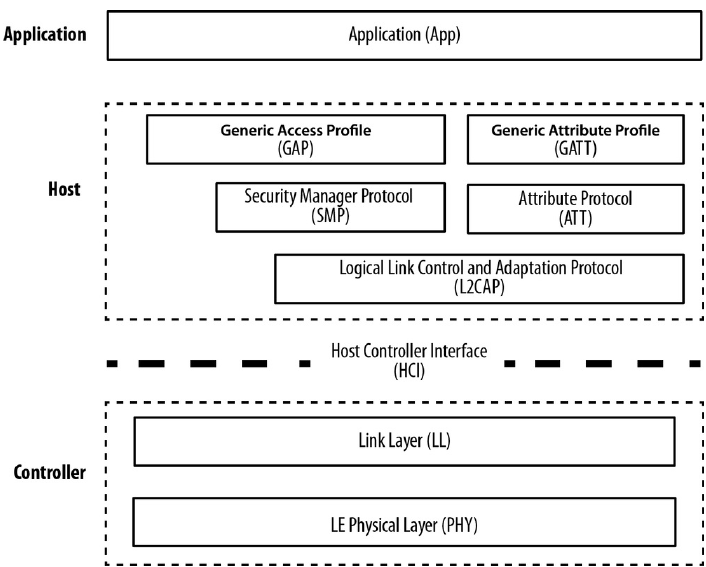
\includegraphics[width=0.6\linewidth]{\figdir/BLE_Protokolstack}
	\caption{\ac{ble} Protokollstack \cite[Seite 16]{Townsend14:GSB}}
	\label{FIG:protokollstack}
\end{figure}

\noindent Die Architektur von \ac{ble} geht aus dem Protokollstack hervor. Dieser ist in Abbildung \ref{FIG:protokollstack} dargestellt. Besonders auffällig ist die Untergliederung in drei Ebenen. Der "`Controller"' stellt dabei den hardwarenähesten Bereich dar. Hier befinden sich die zwei Layer "`LE Physical"' und "`Link"'.\\

\noindent Diese beiden Protokolle sind in einer Großzahl von Gerätearchitekturen beheimatet. Das Physical Layer ist dafür vorgesehen, digitale Signale (Bitfolgen) in analoge umzuwandeln. Dieser Schritt wird benötigt, um die \ac{ble} Signale für etwaige Empfänger zugänglich zu machen. Natürlich werden im Physical Layer auch empfangene analoge Signale in digitale umgewandelt. Dieser werden dann im Protokollstack nach oben ins Link Layer weitergereicht. Im Fall von \ac{ble} ist die Schnittstelle für das Senden der analogen Signale die Luft. \ac{ble} sendet dafür im Frequenzbereich 2,4GHz bis 2,4835GHz. Diesen Bereich teilt sich das Protokoll mit anderen Technologien wie beispielsweise Wifi. Um Kollisionen zu vermeiden teilt \ac{ble} den Bereich in 40 Kanäle auf und wechselt während der Verbindung in regelmäßigen Abständen oder bei Übertragungsproblemen den Kanal. Dieser Ansatz nennt sich Frequency Hopping Spread Spectrum \cite[Seite 16f]{Townsend14:GSB}.\\      

\noindent Das Link Layer unterscheidet sich in seiner Funktionsweise nicht großartig von dem anderer Kommunikationsprotokolle. Hier werden die Nachrichten die für das  Versenden aus den oberen Schichten ankommen in Pakete gepackt und an das Physical Layer weitergereicht. Dieser Prozess ist für ankommende Pakete natürlich vice versa \cite[Seit 194]{Tanenbaum14:CN}. Die Besonderheit ist die Festlegung der Paketgröße von \ac{ble} durch das Link Layer. Seit Version 4.2 ist eine Payload von bis zu 251 Byte pro Paket möglich \cite{Gupta20:WWW}. Zum Vergleich bei WLAN (IEEE 802.11) kann ein Paket bis zu 2312 Byte groß sein \cite[Seite 233]{Gessler15:WNN}. Daraus lässt sich schließen, dass \ac{ble} einen weitaus geringeren Datendurchsatz als WLAN hat. Allerdings liefert \ac{ble} wiederum andere Vorteile. Auf diese wird in Kapitel \ref{s:vergleich} näher eingegangen.\\

\noindent Das Herzstück des \ac{ble} Protokollstacks bilden die beiden Profile \ac{gap} und \ac{gatt}. Diese befinden sich wie in Abbildung \ref{FIG:protokollstack} zu erkennen im Host Bereich der Architektur. Die beiden Protokolle bilden die Schnittstelle zur tatsächlichen Anwendung mit welcher der Nutzer interagiert.\\

\noindent Das \ac{gap} ist dafür vorgesehen sämtliche Parameter der Verbindung zwischen den Geräten zu verwalten. Vom Verbindungsaufbau bis hin zur Kommunikation werden sämtliche Funktionen von diesem Profil bereitgestellt und abgehandelt.\\

\noindent Im Zuge der jeweiligen Konfiguration kann ein Gerät in \ac{ble} eine der folgenden vier Rollen annehmen:
\begin{itemize}
	\item{Broadcaster (Keine Verbindung)}
	\item{Observer (Keine Verbindung)}
	\item{Central (Verbindung)}
	\item{Peripheral (Verbindung)}
\end{itemize}   

\noindent In \ac{ble} ist es nicht festgeschrieben, dass Geräte ein Verbindung eingehen müssen um Informationen zu erhalten. Die Rollen des Broadcasters und Observers sind sogar ausschließlich ohne feste Verbindung zwischen den Geräten vorgesehen. Diese Funktion wird im allgemeinen gerne von \ac{ble} Beacons verwendet.\\

\noindent Ein Gerät welches als Broadcaster definiert ist sendet dauerhaft einen bestimmten Datensatz. Dabei ist zu keinem Zeitpunkt klar, ob Geräte in Reichweite sind, welche den Datensatz empfangen. Ein Gerät welches diese Daten lesen kann muss als Observer konfiguriert sein. Ein solcher scannt die drei Advertisement Kanäle von \ac{ble} dauerhaft nach Broadcastnachrichten. Falls er eine erhält ließt er diese und verwendet sie. Wichtig ist hierbei, dass der Observer keine Antwort auf eine Nachricht sendet.\\  

\noindent Sollte ein Gerät allerdings eine Verbindung eingehen, dann muss dieses als Central konfiguriert sein. Dies ist die gängigste Form des \ac{ble} Gerätes. So ist beispielsweise jedes Smartphone in der Regel als Central konfiguriert und kann Verbindungen zu Peripherals wie zum Beispiel \ac{ble} Kopfhörern aufnehmen. Dabei ist ein Central in der Regel sogar in der Lage mehrere Verbindungen zu selben Zeit einzugehen.\\

\noindent Ein Peripheral wiederum ist das Gegenstück zum Central, welches seine Verbindungsbereitschaft an sämtliche Geräte in Reichweite signalisiert. Im Fall einer aktiven Verbindung übernimmt das Central die Steuerung des Gerätes unter Berücksichtigung des Funktionsumfangs des Peripherals \cite[Seite 34]{Usama17:BBS}.\\

\noindent Das \ac{gap} ermöglicht es einem \ac{ble} Gerät zusätzlich seine Sichtbarkeit und Verbindungsbereitschaft gegenüber anderen Geräten über die Advertisement Kanäle mitzuteilen. Dafür wird auf dem Gerät ein Modus eingestellt welcher anschließend an alle Geräte in Reichweite mitgeteilt wird. Ein Modus ist dabei eng mir der Geräterolle verbunden. Ein Gerät kann folgende Modi annehmen \cite[Seite 35]{Townsend14:GSB}:
\begin{itemize}
	\item{Broadcast (Rolle: Broadcaster)}
	\item{Nicht zu entdecken (Rolle: Peripheral)}
	\item{Eingeschränkt zu entdecken (Rolle: Peripheral)}
	\item{Normal zu entdecken (Rolle: Peripheral)}
	\item{Nicht verbindbar (Rolle: Alle)}
	\item{Verbindbar (Rolle: Central, Peripheral)}
\end{itemize}   

\noindent Im \ac{gatt} wird definiert, ob es sich bei dem Gerät um einen Client oder Server handelt. Zweiterer verarbeitet die Kommunikationsanfragen des Clients und liefert die gewünschten Antworten oder führt entsprechende Aktionen aus. Der Server ist in der Regel ein Peripheral auf dem Services hinterlegt sind \cite[Seite 30]{Usama17:BBS}. Welche das sind und was für eine Aktion mit diesen verbunden ist wird in der Regel durch die Nutzeranwendung festgelegt. Der Client ist dementsprechend ein Central, welches die gesamte Verbindung steuert. Jeder Service verfügt über einen \ac{uuid}. Mit diesem kann der Client eine gezielte Anfrage auf den entsprechenden Service tätigen.\\    

\noindent An oberster Stelle des Protokollstacks befindet sich die Nutzeranwendung. Diese ist nach dem entsprechenden Use Case programmiert und variiert von Anwendung zu Anwendung. Ausschließlich der Stack unterhalb ist für alle Applikationen gleich.\\

\subsection{Kommunikation}
\label{ss:funktionsweise:kommunkation}

\noindent Nachdem in Kapitel \ref{ss:funktionsweise:protokollstack} der Aufbau von \ac{ble} erläutert wurde, wird nun in dem folgenden Kapitel auf die Anwendung der Technologie eingegangen. Dabei wird besonders auf den Verbindungsaufbau durch das Advertisement und den Nachrichtenaustausch der stehenden Verbindung eingegangen.\\

\noindent Die Advertisement Funktion in \ac{ble} kann für zwei Szenarien verwendet werden. Zum einen die Signalisierung der Verbindungsbereitschaft. Zum anderen den Broadcast von Daten in der Rolle des Broadcasters (vgl. \ref{ss:funktionsweise:protokollstack}).\\

\noindent Von den 40 Kanälen, in die der \ac{ble} Frequenzbereich unterteilt ist (siehe Kapitel \ref{ss:funktionsweise:protokollstack}), sind drei für das Advertisement reserviert. Diese befinden sich in den Bereichen 2,402 - 2,404GHz, 2,426 - 2,428Ghz und 2,48 - 2,482GHz. Dabei sind sie mit den Nummern 37 - 39 belegt \cite[Seite 16]{Townsend14:GSB}.\\

\noindent Eine Advertisement Nachricht beinhaltet weiterhin ein Header Feld, welches die Paketadressierung regelt. So kann ein Gerät eine der folgenden vier Advertisement Nachrichten an Geräte in Sendereichweite senden \cite[Seite 22]{Townsend14:GSB}:
\begin{itemize}
	\item{ADV\_IND: Allgemeine Mitteilung der Verbindungsbereitschaft}
	\item{ADV\_DIRECT\_IND: Zielgerichtete Mitteilung der Verbindungsbereitschaft}
	\item{ADV\_SCAN\_IND: Allgemeine Mitteilung der Anwesenheit des Gerätes}
	\item{ADV\_NONCONN\_IND: Allgemeine Mitteilung der Verbindungsunverfügbarkeit}
\end{itemize} 

\begin{figure}[!b]
	\centering
	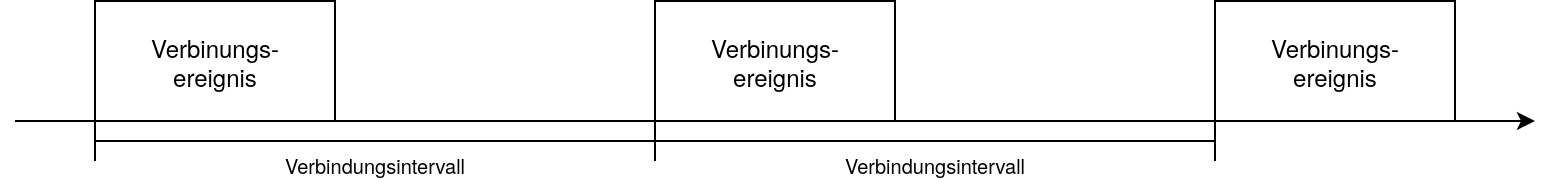
\includegraphics[width=0.8\linewidth]{\figdir/ConEv}
	\caption{Zeitlicher Ablauf einer \ac{ble} Verbindung \cite[Seite 22]{Townsend14:GSB}}
	\label{FIG:ConEv}
\end{figure}

\noindent Eine Verbindung in \ac{ble} besteht aus einer Reihe sogenannter Verbindungsevents. Ein solches wird über drei Parameter definiert welche in den anfänglichen Advertisement Nachrichten vereinbart werden. In Abbildung \ref{FIG:ConEv} ist zu erkennen, wie eine \ac{ble} Verbindung, in zeitlicher Abfolge, abläuft.\\

\noindent Der erste Parameter ist das Verbindungsintervall. Wie aus Abbildung \ref{FIG:ConEv} hervorgeht ist eine Verbindung in derartige Verbindunsintervalle unterteilt. Diese legen die Zeit zwischen den Verbindunsereignissen fest. Dabei sind Werte zwischen 7,5ms und 4s möglich. Kürzere Intervalle bedeuten allerdings einen höheren Energieverbrauch. Ein Verbindungsereignis liegt im Intervall und kann somit maximal so lange wie dieses dauern. Die anderen beiden Parameter legen fest, wann eine Verbindung abbricht, beziehungsweise beendet wird.\\ 

\noindent \ac{ble} ist in seiner Rolle als energiesparsames \ac{iot} Protokoll darum bemüht die als Peripheral eingesetzten Server möglichst Energieeffizient zu betreiben. Daher kann ein derartiges Gerät mehrere Verbindungsevents aussetzen, wenn derzeitig keine Daten zu senden oder empfangen sind. Der Parameter "`Slave Latency"' legt dabei die Anzahl der überspringbaren Ereignisse fest.\\

\noindent Den Zeitpunkt ab welchem eine Verbindung für Beendet erklärt wird, legt der Parameter "`Connection Supervision Timeout"' fest. Dieser legt den Zeitraum fest, der zwischen dem Austausch zweier Datenpakete verstreichen darf. Bei Überschreitung dieses Wertes wird die Verbindung aufgelöst \cite[Seite 22f]{Townsend14:GSB}.\\

\subsection{Anwendungsszenarien}
\label{ss:funktionsweise:anwendungen}

\noindent Die Bluetooth \ac{sig} stellt auf ihrer Website eine Vielzahl verschiedener Anwendungsmöglichkeiten für das Protokoll \ac{ble} vor. Dabei werden vier Hauptkategorien genannt, auf welche sich \ac{ble} konzentriert. Die im Alltag gebräuchlichsten sind dabei das Streamen von Audio und die Datenübertragung. Zusätzlich gibt es allerdings auch noch Positionsservices und das Aufspannen eines Netzwerkes zwischen mehreren \ac{ble} Geräten \cite{BLU20:WWW}.\\

\noindent Seit einigen Jahren steigt die Anzahl der Endnutzer, die statt des herkömmlichen Kabelgebundenen Kopfhörer auf die kabellose Alternative wechseln. Mit der Veröffentlichung des Bluetooth Standards 5.0 wurde dieser Use Case mit \ac{ble} enorm gefördert. Neben Kabellosen Kopfhörern bilden auch Lautsprecher und Mediensysteme in Fahrzeugen interessante Use Cases seitens Bluetooth.\\

\noindent Die Möglichkeit der Datenübertragung ist die Basis des gesamten \ac{ble} Stack. Neben Audio Dateien gibt es eine Vielzahl anderer Anwendungsfälle, wie beispielsweise Kabellosen Tastaturen oder Mäuse. Auch neuere Technologien wie Fitnesstracker oder Smart Watches erfreuen sich in den letzten Jahren immer größerer Beliebtheit. So sind die Umsatzzahlen im Verkauf von Smart Watches laut Heise Online, im Vergleich zum Jahr 2019, dieses Jahr um 20 Prozent gestiegen \cite{HEI20:WWW}. \ac{ble} wird in diesem Fall Verwendet um die von den jeweiligen Peripherals erhobenen Fitness oder Gesundheitsdaten an das Smartphone als Central Gerät zu übertragen.\\

\noindent Ein großes Problem der vergangenen Jahre war die Positionsbestimmung in geschlossenen Räumen. Im Freien ist diese durch Satellitenkommunikation möglich. In Gebäuden kann diese Technologie allerdings auf Grund zu großer Ungenauigkeiten und der fehlenden direkten Verbindung nicht gewährleistet werden. Für dieses Problem liefert \ac{ble} mit Hilfe der Broadcaster Rolle eine Lösung. Dafür gibt es ein breites Spektrum an Möglichkeiten. Dieses Reicht von Indoor Navigation über die Positionsüberwachung von Gegenständen oder Personen bis hin zu Informationsystemen. Letztere stellen \ac{ble} Broadcaster dar, die bei Annäherung eines Observers nützliche Informationen senden. Dies kann beispielsweise in einem Museum sehr nützlich sein. Auch im Hinblick auf eine SAP Anbindung bietet die Indoor Positionsbestimmung mittels \ac{ble} eine praktische Lösung. Diese kann beispielsweise zur Überwachung von autonomen Fahrzeugen in der Fertigung genutzt werden.\\          

\noindent Der vierte große Bereich, welchen die Bluetooth \ac{sig} besonders hervorhebt, behandelt die Vernetzung verschiedener \ac{ble} Geräte. Dieser Bereich ist vor Allem im Hinblick an SAP besonders interessant, da er sich mit der Kontrolle, Überwachung und Automatisierung ganzer Systeme befasst. Die Bluetooth \ac{sig} Verspricht unter anderem Lösungen zur Überwachung und Steuerung von Temperatur, Feuchtigkeit und Raumbelegungen in Gebäuden. Diese sollen das Ziel verfolgen die Produktivität der Angestellten zu steigern.\\   

\section{Schnittstellenbeschreibung}
\label{s:interface} 

\noindent Nachdem in Kapitel \ref{s:funktionsweise} auf die Funktionsweise von \ac{ble} eingegangen und die resultierenden Möglichkeiten erläutert wurden, wird im nachfolgenden Kapitel auf die Anbindung des Kommunikationsprotokolls an SAP eingegangen. Dabei liegen die Schwerpunkte auf Schnittstelle, Administration und daraus resultierenden Möglichkeiten für den Anwender.\\

\subsection{Komponenten SAP Leonardo IoT}
\label{ss:interface:sap}

\begin{figure}[!b]
	\centering
	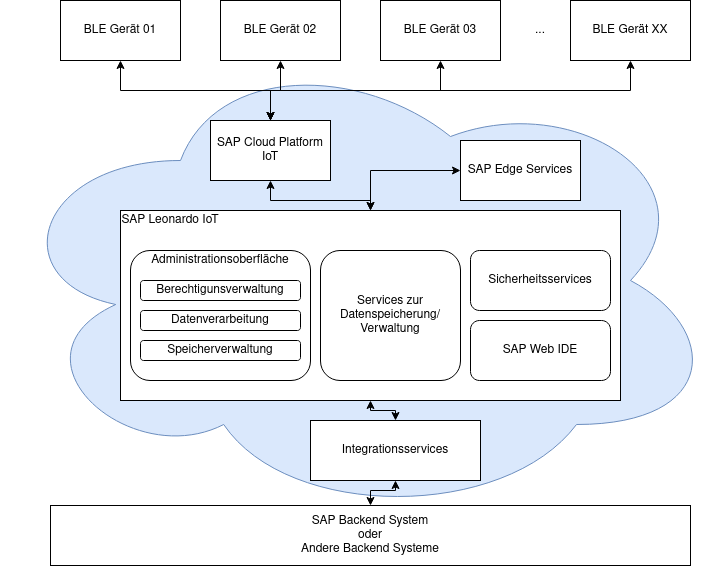
\includegraphics[width=1\linewidth]{\figdir/Interface}
	\caption{Überblick über die SAP \ac{iot} Architektur \cite[Seiten 117, 164, 181, 184, 201, 208, 221]{Holtschulte20:IOS}}
	\label{FIG:Interface}
\end{figure}

In Kapitel \ref{ss:grundlagen:sap} wurde auf die Marke SAP Leonardo verwiesen, welche unter anderem eine \ac{iot} Schnittstelle liefert. Ein Überblick über diese Schnittstelle findet sich in Abbildung \ref{FIG:Interface}. Aus dieser geht hervor, dass sich die gesamte Anwendung in der SAP Cloud befindet.\\

\noindent Den Kern bildet hier die Unterkategorie von SAP Leonardo mit dem Beinamen \ac{iot}. Dieser Teil ist mit einer \ac{gui} buchbar, die neben einer Administrationsoberfläche, auf die in Kapitel \ref{ss:interface:admin} näher eingegangen wird, Services für Datenverwaltung und IT Sicherheit liefert. Zusätzlich bietet SAP eine voll Funktionsfähige Web \ac{ide}.\\

\noindent Die Datenverwaltung in SAP Leonardo \ac{iot} soll den Nutzer dabei unterstützen relevante Daten die von etwaigen \ac{iot} Geräten empfangen wurden gewinnbringend zu verwerten. Hierfür können Regeln und Aktionen definiert werden, wie die Daten behandelt werden sollen. Da auf verschieden Daten unterschiedlich schnell zugegriffen werden muss, bietet SAP auch hierfür verschieden Speicherbereiche an, welche sich entsprechend im Preis unterscheiden \cite[Seite 173]{Holtschulte20:IOS}. Wenn ein sehr schneller Speicherzugriff notwendig ist, dann liefert die Hot Storage Funktion die benötigte Geschwindigkeit. Allerdings ist diese auch am teuersten. Weitere Speicherzugriffsvarianten die das SAP \ac{iot} Paket enthält sind der Warm und Cold Storage. Bei der Warm Storage Variante sind schnelle aber nicht so häufige Speicherzugriffe notwendig. Die Cold Storage Variante hingegen speichert Daten die über lange Zeit nicht mehr benötigt werden. Entsprechend sind langsame Speichermedien vollkommen ausreichend. Diese Art des Speicherzugriffs nennt man auch Mutli Temperature Datenverwaltung \cite[Seite 118f]{Holtschulte20:IOS}. Falls eine langfristigere Speicherung oder eine Weiterverwendung der Daten benötigt werden, können SAP HANA oder Big Data Services gebucht werden, welche dies übernehmen \cite[Seite 173]{Holtschulte20:IOS}.\\    

\noindent Um die Sicherheit der Anwendung zu gewährleisten bietet die SAP Cloud Platform diverse Services zur Authentifizierung. In der Regel weißt man dabei seine Identität über eine Drittanbieter Software aus. Darüber hinaus liefert die Anwendung SAP Cloud Platform Cockpit die Möglichkeit Nutzern verschiedene Rollen zuzuweisen \cite[Seite 176ff]{Holtschulte20:IOS}.\\

\noindent Um die SAP Cloud mit einem Backend System zu verbinden wird der \ac{cpi}  Service verwendet. Dabei ist zu beachten, das auch nicht SAP Systeme über diesen Service mit der Cloud kommunizieren können. Der Service ist mit dem SAP Cloud Paket buchbar \cite[Seite 146]{Holtschulte20:IOS}.\\

\noindent Um ein \ac{iot} Gerät mit SAP Leonardo \ac{iot} anzubinden gibt es zwei Möglichkeiten. Zum einen den Service SAP Cloud Platform \ac{iot} und zum anderen die Verwendung sogenannter Edge Services. Erster ist die Standardlösung welche von SAP angeboten wird. Über diesen Service lassen sich angeschlossene Geräte unter dem Reiter Device Management verwalten und neue hinzufügen. Im Reiter Component Management wiederum kann der Gateway konfiguriert werden, über den die Kommunikation mit dem jeweiligen Gerät abgehandelt wird \cite[Seite 200f]{Holtschulte20:IOS}. Hierbei gibt es folgende drei mögliche Gateways \cite[Seite 117]{Holtschulte20:IOS}:
\begin{itemize}
	\item{\ac{opc}}
	\item{\ac{mqtt}}
	\item{\ac{http}}
\end{itemize}
Über den Reiter Processing kann anschließend definiert werden, auf welche Weiße ankommende Daten von \ac{iot} Geräten verarbeitet werden. Zusätzlich können Daten sogar für einen Zeitraum X aufbewahrt werden \cite[Seite 205]{Holtschulte20:IOS}.\\

\noindent Sollte das \ac{iot} Gerät, welches an SAP angebunden werden soll, über keine Möglichkeit verfügen an einen der drei SAP Cloud Platfrom \ac{iot} Gateways angeschlossen zu werden, wird ein SAP Edge Service benötigt. Ein solcher kommt darüber hinaus zum Einsatz, wenn es nötig ist die Daten, welche das \ac{iot} Gerät ermittelt, möglichst schnell zu verwerten und auf diese zu reagieren. Dafür wird direkt am \ac{iot} Gerät ein Service installiert, welcher über Konfigurationsmöglichkeiten verfügt um entsprechende Regeln anzuwenden. Da die Latenz zur Cloud in diesem Fall viel zu hoch ist wird ein SAP Edge Service nicht an die SAP Cloud Platform \ac{iot} angebunden. Ein solcher Service verfügt selbst über eine Liste von Gateways um direkt mit dem \ac{iot} Gerät und SAP Leonardo \ac{iot} zu kommunizieren. Dabei erweitert SAP die Liste an Möglichen Gateways zu \ac{iot} Geräten um die Protokolle Sigfox, FILE, Modbus, Constrained Application Protocol (CoAP) und Simple Network Management Protocol (SNMP). Um auf bestimmte Szenarios reagieren zu können sind über einen SAP Edge Service folgende integrierte Services verfügbar\cite[Seite 229ff]{Holtschulte20:IOS}:
\begin{itemize}
	\item{Essenzielle Business Funktionen: Synchronisation mit SAP Geschäftssystemen}
	\item{Streaming: Analyse und Verarbeiten der \ac{iot} Rohdaten}
	\item{Persistenz: Vorübergehende Speicherung von Daten auf dem SAP Edge Service}
	\item{Predictive Analytics: Analyse der Daten mittels künstlicher Intelligenz}
\end{itemize}   

\subsection{Administration SAP Leonardo IoT}
\label{ss:interface:admin}

\noindent Der Administrationsbereich von SAP Leonardo \ac{iot} verfügt über einen Arbeitsbereich welcher neben diversen Administrationsfunktionen zusätzlich Möglichkeiten zur Modellierung und Simulation in Form eines digitalen Zwillings der angeschlossenen \ac{iot} Systeme bietet. Zur Administration der Schnittstelle liefert die \ac{gui} folgende Möglichkeiten:
\begin{itemize}
	\item{Rollenverwaltung und Zuweisung}
	\item{Tenantverwaltung}
	\item{Paketverwaltung}
	\item{Definition von Regeln und Aktionen}
\end{itemize}

\noindent Im Bereich "`Trust Configurator"' lassen sich den jeweiligen Benutzern des Systems ihre Rollen zuweisen. Dies wird, abhängig von deren Identity Provider, über deren Email oder entsprechen andere Identifikatoren abgehandelt \cite[Seite 209f]{Holtschulte20:IOS}. Um Zuweisungen vornehmen zu können benötigt der Nutzer Administrationsrechte. Diese erhält er über einen bei der Buchung durch SAP ausgestellten Tenant. Dieser definiert die Rolle des Tenant Administrators und entspricht dem Systemadministrator. Er verfügt über folgende drei gesonderte Administrationsbereiche \cite[Seiten 220 - 221, 223]{Holtschulte20:IOS}:
\begin{itemize}
	\item{Objektberechtigungen: Anlegen von Berechtigungen für Objekt- und Personengruppen}
	\item{Personen: Anlegen und Unternehmenszuweisung von Personen}
	\item{Unternehmen: Anlegen von Unternehmen zur Personenzuweisung}
\end{itemize}

\noindent Ein weiterer wichtiger Bereich der Administration ist die Definition von Regeln und Aktionen. Ein Beispiel für eine Regel wäre die Messung eines zu hohen Temperaturwertes mittels \ac{iot} Gerätes. Regeln dienen daher der Definition von Grenzwerten, welche bei Über- oder Unterschreitung eine Aktion erfordern. Um in SAP Leonardo \ac{iot} eine Regel einzuführen muss zunächst ein Kontext definiert werden. Dieser beschreibt die Eigenschaft des Geräteteils, für welche die Regel definiert ist. Im vorigen Beispiel wäre der Kontext die Temperaturmessungseinheit des Gerätes. In diesem Kontext lassen sich Regeln in einer der drei Kategorien Streaming Cloud, Streaming Hybrid, oder Eingeplant definieren. Streaming Cloud Regeln werden für Ereignisse definiert, welche bei Geräten auftreten, die über die SAP \ac{iot} Platform angeschlossen sind. Streaming Hybrid Daten sind wiederum das Pendant für die Edge Services. Eingeplante Regeln werden prüfen in bestimmten Abständen oder zu selbst definierten Zeitpunkten ob in den letzten X Minuten eine Regelverletzung erkannt wurde. Diese finden bei nichtkritischen Komponenten Verwendung. Für jede Regel lässt sich nun eine Aktion definieren, welche bei deren Verletzung ausgeführt wird. Sämtliche Einstellungen für Regeln und Aktionen finden sich unter dem Reiter "`IoT-Regeln und Aktionen"' im Administrationspanel \cite[Seite 224ff]{Holtschulte20:IOS}.\\   

\subsection{Bluetooth Low Energy mit Message Queuing Telemetry Transport (MQTT)}
\label{ss:interface:ble}

\begin{figure}[!b]
	\centering
	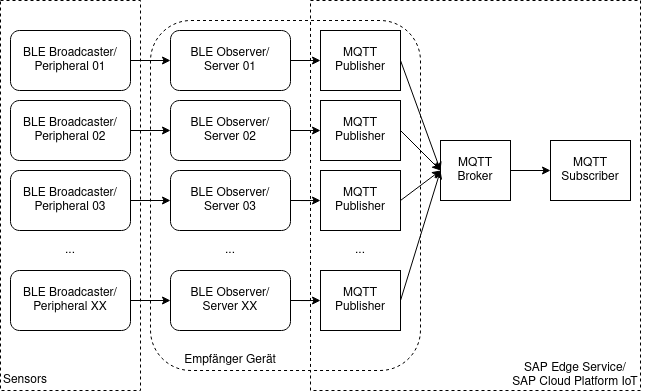
\includegraphics[width=0.8\linewidth]{\figdir/ble_mqtt}
	\caption{Zusammenhang zwischen \ac{ble}, \ac{mqtt} und SAP \cite[Seite 3f]{Zivkovic20:MQTT} \cite[Seite 230f]{Holtschulte20:IOS}}
	\label{FIG:mqtt}
\end{figure}

\noindent Bei \ac{ble} handelt es sich um ein Protokoll, welches nicht über IP Adressen, also das Internet, kommuniziert. Da SAP Leonardo \ac{iot} jedoch eine Lösung in der SAP Cloud ist wird eine Schnittstelle benötigt, um Daten zwischen Endgerät und Cloud zu transportieren. Zusätzlich verfügen die SAP \ac{iot} Lösungen über kein \ac{ble} Modul, welches direkt mit einem entsprechenden Endgerät kommunizieren kann. SAP verfügt allerdings sowohl in der SAP Cloud Platform \ac{iot} als auch in den SAP Edge Services über einen \ac{mqtt} Gateway. Ein solcher ist in der Lage Daten über einen sogenannten Publisher zu empfangen und dann über das Internet an die entsprechenden Stellen weiterzuleiten.\\

\noindent In Abbildung \ref{FIG:mqtt} sind die verschiedenen Verbindungsabschnitte zwischen \ac{ble} und SAP dargestellt und in einen Zusammenhang gebracht. Die \ac{ble} Sensoren/Geräte nehmen entweder die Rolle eines Boradcasters oder Peripherals ein. Die Bedeutung dieser Rollen findet sich in Kapitel \ref{ss:funktionsweise:kommunkation}. Zum Empfangen von Nachrichten wird ein Gerät benötigt, welches über ein \ac{ble} Modul verfügt und entweder als Observer oder Central konfigurierbar ist. Dieses Gerät muss zusätzlich über eine Internetverbindung verfügen. Zur Anbindung an SAP wird auf dem Gerät eine Software installiert, welche \ac{mqtt} unterstützt. Diese Software wird als Publisher konfiguriert. Dieser Publisher kann dann als solcher am SAP \ac{mqtt} Broker angelegt werden. Auf SAP Seite leitet der SAP \ac{mqtt} Broker dann sämtliche an ihn veröffentlichten Daten an etwaige konfigurierte Stellen weiter. Diese Stellen werden im \ac{mqtt} Kontext als Subscriber benannt.\\

\noindent Das \ac{mqtt} Protokoll besteht grundlegend aus folgenden drei Komponenten:
\begin{itemize}
	\item{Broker: Verwaltung von Publishern und Subscribern}
	\item{Publisher: Veröffentlichung von Daten am Broker}
	\item{Subscriber: Empfangen von Daten zu abonnierten Topics}
\end{itemize}
Aus Abbildung \ref{FIG:mqtt} geht hervor, dass sämtliche Kommunikation zwischen dem Nachrichtenempfänger (Subscriber) und dem Sender (Publisher) über den Broker verlaufen. Eine Besonderheit bei \ac{mqtt} ist, dass die Publisher und Subscriber nichts voneinander wissen. Dies liegt an der Topic Funktion von \ac{mqtt}. Ein Topic beschreibt ein Thema, welches der Broker kennt. Der Publisher gibt an, dass er auf ein bestimmtes Thema Nachrichten sendet. Ein Subscriber wiederum abonniert ein Topic. Wenn nun ein Publisher eine Nachricht an dieses Topic veröffentlicht, benachrichtigt der Broker sämtliche Subscriber das eine Nachricht veröffentlicht wurde und übermittelt diesen die veröffentlichte Nachricht. Dabei können auch mehrere Publisher auf ein Thema Veröffentlichen und mehrere Subscriber ein Thema abonnieren.\\

\noindent Ein Thema im \ac{mqtt} Kontext gliedert sich hierarchisch in einer Baumstruktur. Sollte beispielsweise ein \ac{ble} Sensor dafür verwendet werden in einem Logistikzentrum die Position eines autonomen Transportfahrzeuges zu überwachen, dann könnte am Broker ein Topic mit der Hierarchie "`lagerhalle/abschnitt\_c/fahrzeug\_12/position"' angelegt werden, auf welches der entsprechende Publisher veröffentlicht. Ein Subscriber wiederum wäre bemächtigt mit dem Topic "`lagerhalle/abschnitt\_c/+/position"' die Position aller registrierten Fahrzeuge in Abschnitt C der Lagerhalle zu abonnieren \cite{MQTT19:WWW}.\\

\noindent Im konkreten Fall von \ac{ble} und SAP können die Topics über die \ac{gui} der SAP Cloud Platform \ac{iot} oder des SAP Edge Services konfiguriert werden. Die Nachrichten, welche veröffentlicht werden enthalten die Payload im Json Format. Daraus resultiert die Notwendigkeit einer Umwandlung der \ac{ble} Daten in das Json Format auf \ac{ble} Empfänger Seite. Diese muss durch das Empfängergerät vorgenommen werden, bevor die Daten an den Publisher weitergereicht werden. \cite[Seite 247]{Holtschulte20:IOS}.\\ 

\section{Vergleich von Bluetooth Low Energy mit konkurrierenden Protokollen}
\label{s:vergleich} 

\noindent Nach Erläuterung der technischen Rahmenbedingungen für die Anbindung von \ac{ble} Geräten an SAP im vorangehenden Kapitel und der Erklärung der klassischen Anwendungsgebiete in Kapitel \ref{ss:funktionsweise:anwendungen}, stellt sich nun die Frage was \ac{ble} von anderen \ac{iot} Protokollen unterscheidet und wie sich \ac{ble} im Vergleich zu diesen profilieren kann. Um dieser Frage auf den Grund zu gehen, wird im folgenden Kapitel geklärt, welche \ac{iot} Kommunikationsprotokolle mit \ac{ble} konkurrieren und es werden Vor- und Nachteile gegeneinander abgewägt.\\ 

\subsection{WLAN (IEEE 802.11b)}
\label{ss:vergleich:wlan}

\noindent WLAN ist ein Kommunikationsprotokoll, welches wie \ac{ble} im lizenzfreien 2,4 bis 5 GHz Frequenzbereich sendet, aber eine viel höhere Datenrate und Reichweite bietet. Deshalb ist WLAN aktuell das Protokoll mit den meisten Nutzgeräten weltweit \cite[Seite 193f]{Gessler15:WNN}. Dabei gehört es allerdings nicht zur Gruppe der klassischen \ac{iot} Kommunikationsprotokolle, da sämtliche Kommunikation über einen Router läuft, welcher die Geräte miteinander verbindet.\\

\noindent Die hohe Datenrate und Reichweite von WLAN resultiert in einem sehr hohen Energieverbrauch. Ein \ac{ble} Gerät kann hingegen bereits mit geringen Stromquellen versorgt werden. Des weiteren sind die Kosten für \ac{ble} Chiplösungen viel geringer und können einem Unternehmen in hoher Stückzahl viel Geld einsparen. Im Gegensatz zu WLAN ist \ac{ble} ausschließlich im Ad-Hoc Modus verfügbar. Dies ermöglicht die Aufspannung eines dezentrale Funkbetriebes und einer daraus resultierend geringeren Infrastruktur und wiederum eingesparten Kosten in Installation und Instandhaltung \cite[Seite 206]{Gessler15:WNN}.\\

\noindent WLAN bietet zwar auch die Möglichkeit eines Ad-Hoc Modus. Dies bringt allerdings eine aufwändigere Konfiguration mit sich, da jede IP Adresse manuell zugewiesen werden muss. Zusätzlich ist dieser Ad-Hoc Modus ausschließlich ohne Zugriff auf das Internet verfügbar und benötigt auf Grund der WLAN spezifischen Paketgröße dennoch mehr Energie als \ac{ble}. Der WLAN Ad-Hoc Modus bietet deshalb allerdings auch die Möglichkeit einer höheren Datenrate. Um den hohen Stromverbrauch einzuschränken verfügt WLAN über diverse Stromsparfunktionen. Dafür werden einerseits eingeholte Informationen gecached um unnötigen Datenaustausch zu vermeiden. Andererseits werden die Abstände zwischen dem Senden bestimmter Signale verlängert \cite[Seite 240ff]{Gessler15:WNN}.\\ 

\noindent Beide Protokolle arbeiten auf dem selben Frequenzband und sind primär für den Nachrichtenaustausch zwischen zwei Geräten gedacht. Für den Einsatz von WLAN sprechen Datenrate, Reichweite und Zugriff auf das Internet. Nachteil davon ist jedoch die Notwendigkeit einer Infrastruktur und der hohe Energieverbrauch. \ac{ble} kommt hingegen ohne Infrastruktur aus und kann über die Konfiguration verschiedener Rollen selbstständig ein Ad-Hoc Netzwerk aufspannen. Sollten Anhand dieser Punkte noch keine eindeutige Entscheidung zwischen den Protokollen gefällt werden können, sollten die geringeren Kosten für \ac{ble} Geräte in Betracht gezogen werden \cite[Seite 271]{Gessler15:WNN}.\\   

\subsection{ZigBee (IEEE 802.15.4)}
\label{ss:vergleich:zigbee}

\noindent ZigBee ist ein Funkprotokoll, welches eine günstige, ausfallsichere und energiesparsame Vernetzung von \ac{iot} Geräten ermöglicht. Im SAP Kontext besonders interessant sind die Anwendungsgebiete in Medizin-, Gebäude-, und Industrie-Automatisierung. Es basiert auf dem IEEE 802.15.4 Standard \cite[Seite 195]{Gessler15:WNN}.\\  

\noindent ZigBee legt den Hauptaugenmerk auf die Fernsteuerung von einfachen Gebäudeausstattungsgeräten wie beispielsweise Lampen, Lichtschaltern und Heizungen. Das Protokoll sendet Nachrichten aus Energiegründen nur über kurze Distanzen zu benachbarten ZigBee Geräten. Eine hohe Reichweite erreicht das Protokoll durch die Vernetzung der verfügbaren Geräte. Um ein Netz aufzuspannen werden alle Geräte an einem Gateway bekannt gemacht. Dieser wird als Koordinator bezeichnet. Neben diesem beinhaltet ein ZigBee Netzwerk Router und Endknoten. Ein Router gibt dabei alle Nachrichten, welche nicht an in adressiert sind an den nächsten Knoten weiter. Sollte ein Gerät ausfallen oder entfernt werden, wird dies erkannt und eine neue Route zu den verlorenen Geräten wird eingerichtet \cite{ZIG20:WWW}.\\

\noindent Die zugrundeliegende IEEE 802.15.4 Standard benötigt im Vergleich zu \ac{ble} beinahe die doppelte Energie um ein Paket zu übertragen \cite[Seite 4]{Fafoutis16:BOI}. Diesen höheren Energieverbrauch bekommt ZigBee allerdings durch die kurzen Sendedistanzen zwischen den einzelnen Geräten des Netzwerkes und dem senden kleiner Datenpakete unter Kontrolle. Dadurch kann ein ZigBee Gerät trotz des vergleichbar hohen Energieverbrauchs von IEEE 802.15.4 im Hibernation Mode des ZigBee Protokollstacks bis zu mehrere Jahre aktiv sein \cite[Seite 267]{Gessler15:WNN}.\\

\noindent Die Mobilität des ZigBee Protokolls ist durch die Gateway Instanz in Form des Koordinators eingeschränkt. Im Kontext mit SAP fällt dieser allerdings nicht schwer ins Gewicht, da auch für \ac{ble} ein Gateway für \ac{mqtt} eingerichtet werden muss. Dennoch verfügt ZigBee über keinen Ad-Hoc Modus wie in \ac{ble} in vollem Umfang einsetzt. Im Bezug auf Signalstörungen der beiden Protokolle über mehrere Räume hinweg sind ist die Stabilität der Übertragungen beinahe Identisch \cite[Seite 6]{Fafoutis16:BOI}.\\

\noindent ZigBee ist somit ein Protokoll, welches eine gute alternative zu \ac{ble} bietet. Allerdings muss die geringe Datenrate des Protokolls in den Auswahlprozess eingebunden werden. ZigBee eignet sich Hervorragend um knappe Befehle an verteilte Systeme zu übertragen. Sollte jedoch eine aufwändigere Kommunikation benötigt werden, stößt ZigBee schnell an seine Grenzen. Somit ist \ac{ble} das funktional Umfangreichere Protokoll, muss sich allerdings im Steuerungsbereich von einfachen Geräten geschlagen geben.\\

\section{Fazit}
\label{s:fazit}

  
%%% Local Variables: 
%%% mode: latex
%%% TeX-master: "thesis.tex"
%%% End: 




%\appendix
%\section{Erster Abschnitt des Anhangs}
\label{a:somelabel}
In diesem Anhang wird \dots 

%%% Local Variables: 
%%% mode: latex
%%% TeX-master: "thesis.tex"
%%% End: 



\bibliographystyle{natger}
\bibliography{thesis}



\end{document}
